% flashcards-title: Structure of eight plus three times four
% flashcards-desc: An addition node joins the number eight to a multiplication node whose children are three and four.
\documentclass[dvisvgm,tikz,border=8pt]{standalone}
\usetikzlibrary{arrows.meta,patterns}

\definecolor{qraNavy}{HTML}{17324D}
\definecolor{qraBlue}{HTML}{2B6CB0}
\definecolor{qraGold}{HTML}{B7791F}
\definecolor{qraPale}{HTML}{EAF2F8}
\definecolor{qraGray}{HTML}{5C6773}

\tikzset{
  qra axis/.style={draw=qraNavy, line width=1.2pt},
  qra tick/.style={draw=qraNavy, line width=1pt},
  qra guide/.style={draw=qraGray, densely dashed, line width=0.8pt},
  qra counter/.style={circle, draw=qraNavy, fill=qraPale, line width=0.9pt, minimum size=7mm, inner sep=0pt},
  qra label/.style={font=\sffamily\bfseries, text=qraNavy},
  qra small label/.style={font=\sffamily, text=qraNavy},
}

\begin{document}
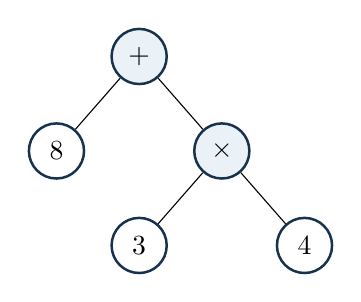
\begin{tikzpicture}[level distance=1.2cm,sibling distance=2.1cm]
  \node[qra counter,fill=qraPale] {$+$}
    child {node[qra counter,fill=white] {$8$}}
    child {node[qra counter,fill=qraPale] {$\times$}
      child {node[qra counter,fill=white] {$3$}}
      child {node[qra counter,fill=white] {$4$}}};
\end{tikzpicture}
\end{document}
